%%%%%%%%%%%%%%%%%%%%%%%%%%%%%%%%%%%%%%%%%%%%%%%%%%%%%%%%%%%%
% Dario Nascimento (dario.nascimento@tecnico.ulisboa.pt)
%
% This file may be distributed and/or modified
%
% 1. under the LaTeX Project Public License and/or
% 2. under the GNU Public License.
%%%%%%%%%%%%%%%%%%%%%%%%%%%%%%%%%%%%%%%%%%%%%%%%%%%%%%%%%%%%%
%%%%%%%%%%%%%%%%%%%%%%%%%%%%%%%%%%%%%%%%%%%%
%%        IST Non-official beamer template
%%%%%%%%%%%%%%%%%%%%%%%%%%%%%%%%%%%%%%%%%%%%%
%% Dário Nascimento - dfrnascimento@gmail.com
%%%%%%%%%%%%%%%%%%%%%%%%%%%%%%%%%%%%%%%%%%%%%
%% ATTENTION: Use xelatex engine instead of
%% pfdlatex due to font changes
%%%%%%%%%%%%%%%%%%%%%%%%%%%%%%%%%%%%%%%%%%%%%

%Comment the following line to compile notes and slides separated
\documentclass{beamer}


\logo{
\includegraphics[width=1.6cm]{logos/logo}}
\usetheme[pageofpages=of,% String used between the current page and the
                         % total page count.
          titleLine=true,% Show a line below the frame title.
          alternativeTitlePage=true,% Use the fancy title page.
          titlePageLogo=logos/logo,% Logo for the first page.
          titlePageSecondLogo=logos/inesc,% the 2nd logo for the first page.
          ]{Lisbon}
       
       



\title{Recovery from Security Intrusions in Cloud Computing}
\author{Dário Nascimento}
\institute{68210 - MERC\\ Instituto Superior Técnico\\ Universidade de Lisboa}
\def\supervisor{Prof. Miguel Pupo Correia}
\date{May 10, 2014}

\begin{document}
\begin{frame}[t,plain]
\titlepage
\note{Boa tarde, sou o Dário Nascimento, aluno 68210 do mestrado de Redes de Comunicação do Instituto Superior Técnico.
Hoje venho apresentar o meu Projecto de tese intitulado de: Recovery from Security Intrusions in Cloud Computing}
\end{frame}

%-------------------------------------------------------------------
%\AtBeginSection[] - if you want the table of contents at begin of every section
\begin{frame}
	\frametitle{Agenda}
	\vskip-25pt
	\tableofcontents
	%\tableofcontents[currentsection] %if you want at begin of every section
	\note{Começarei por introduzir a motivação deste trabalho e as soluções existentes para os problemas deste tópico. De seguida, apresentarei uma solução para os problemas que se encontram por resolver, explicando os seus objectivos e a sua arquitectura. Por fim, serão apresentados os métodos de avaliação da solução proposta e o calendário para a sua execução. Após o dito, irei concluir a minha apresentação.}
\end{frame}

%%%%%%%%%%
% 00:45
%%%%%%%%%%%%%
\section{Motivation}
\begin{frame}[t]{Motivation}
    \vskip-0.2cm
    \textbf{Increasing number of critical applications in Cloud}
	\vskip0.5cm
		\textbf{Intent to compromise:}
	\begin{itemize}
		\setlength{\wideitemsep}{2pt}
		\item Confidentiality
		\item Integrity
		\item Availability
	\end{itemize}
	\vspace{0.5cm}
	\textbf{Intrusion:}
	\begin{itemize}
		\setlength{\wideitemsep}{2pt}
		\item Intentional vulnerability exploitation
		\item Malicious fault
	\end{itemize}

	\vspace{0.5cm}
	Recover the application \textbf{integrity} to prevent \textbf{losses}

	\note{
	As aplicações web estão expostas a um ambiente não confiável em que as aplicações e os sistemas através dos quais estas são disponibilizados, sofrem ataques constantemente. Os ataques visam explorar vulnerabilidades para comprometer a confidencialidade, integridade e disponibilidade da aplicação. Se bem sucedido, o ataque provoca uma falta maliciosa.

	Importa relembrar que a disponibilidade do aplicação depende também da sua integridade. Se os dados corrompidos forem expostos aos utilizadores, ocorre um erro, e a aplicação falha, ficando indesponível. Uma aplicação indisponível e/ou com os dados corrompidos não só é inútil como também pode causar enormes prejuízos quer aos providers pela quebra do service level agreement, SLA, quer aos clientes que dependem da aplicação.}
\end{frame}

%%%%%%%%%%
% 01:45
%%%%%%%%%%%%%

%-------------------------------------------------------------------
\begin{frame}[t]{Motivation}
	\begin{center}
		\begin{figure}
		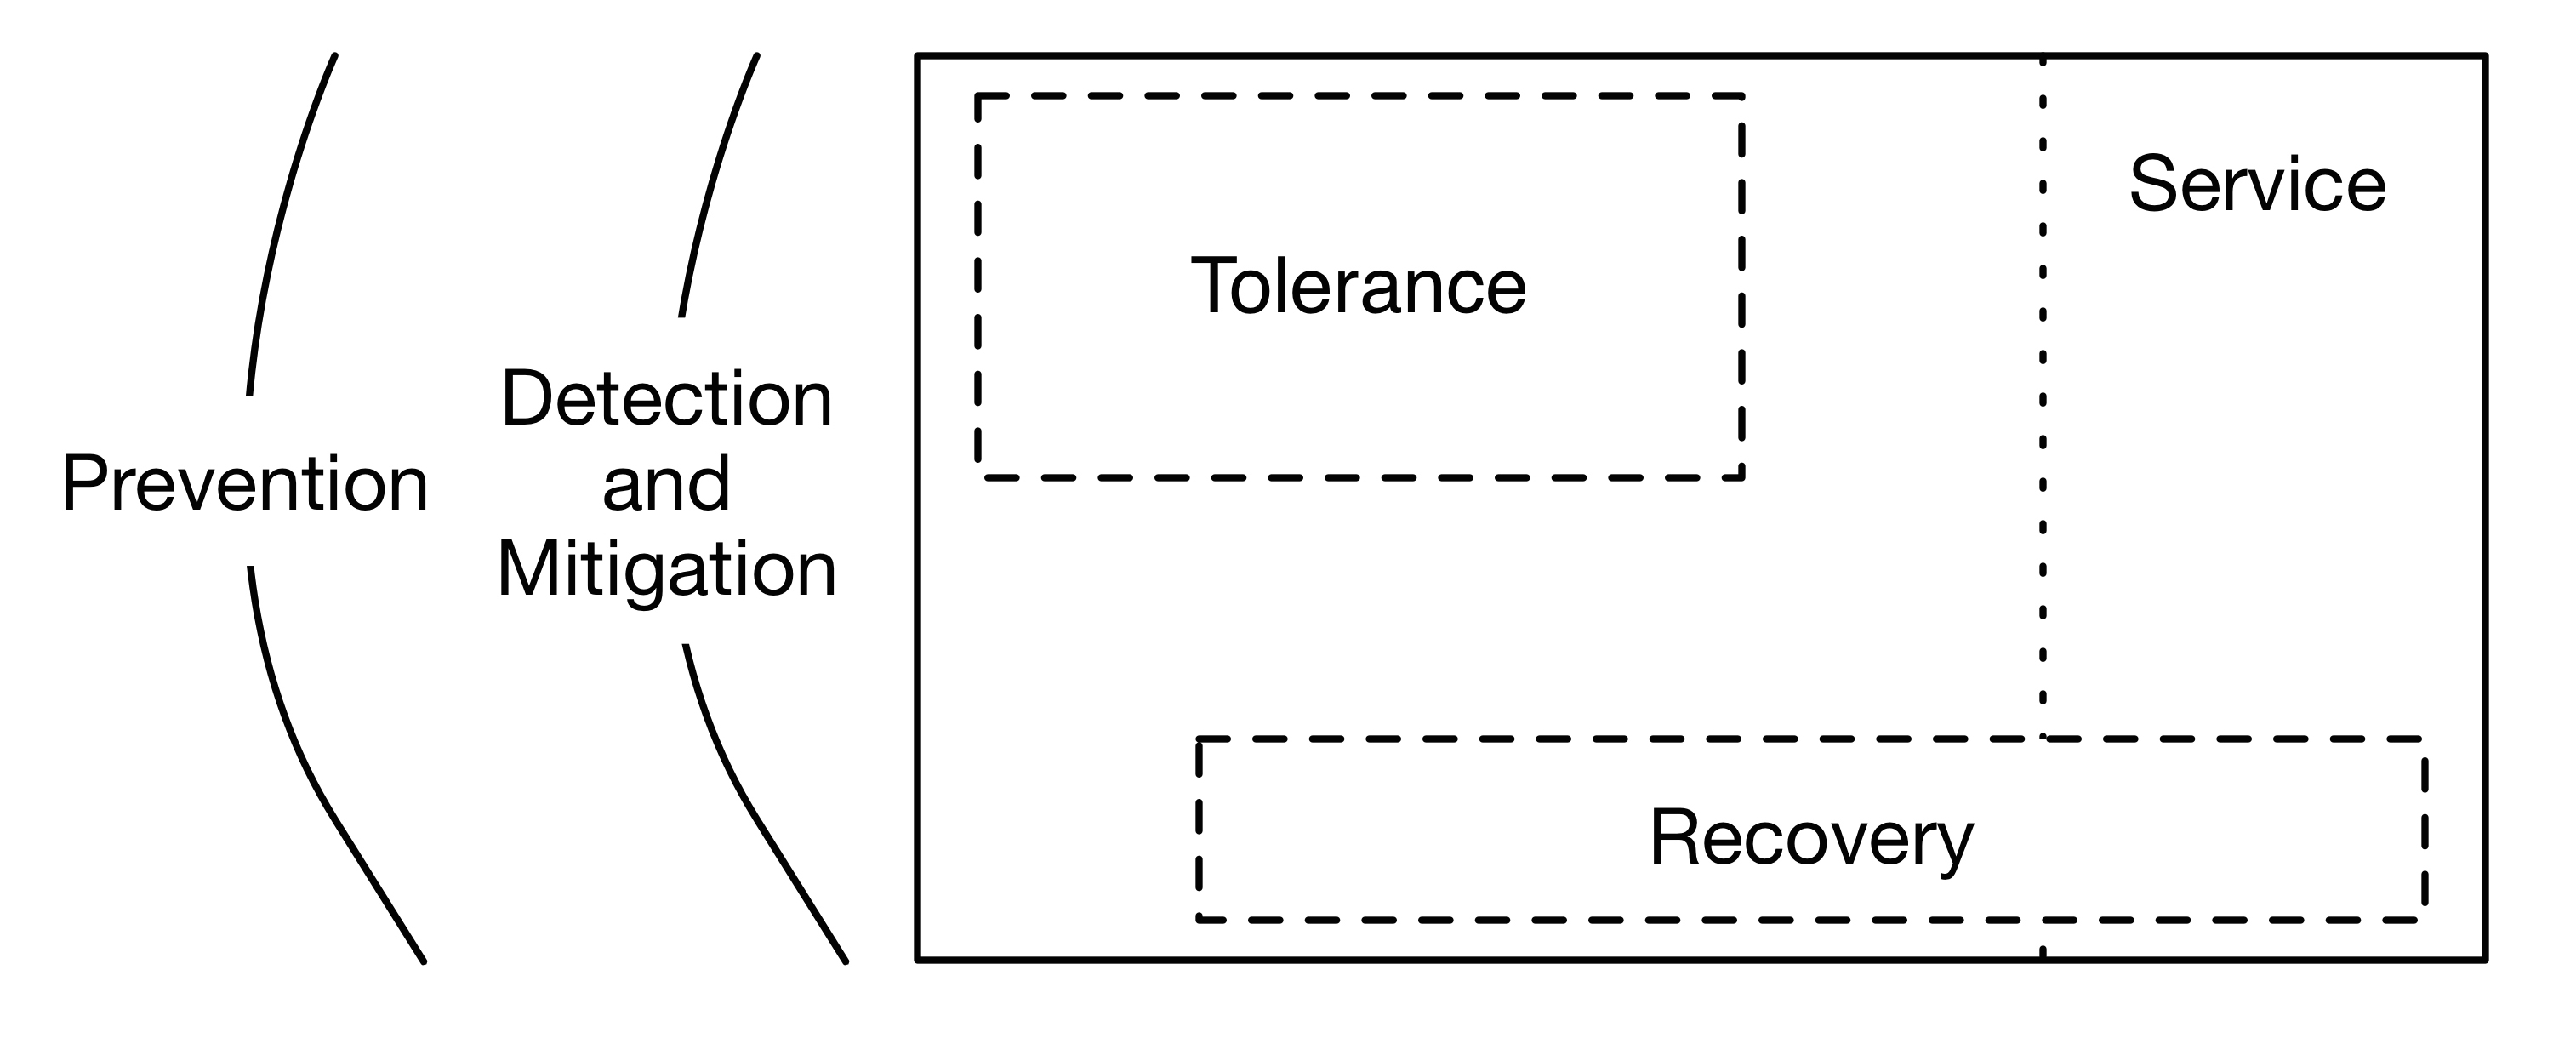
\includegraphics[width=0.8\textwidth]{img/ie0}
	 \end{figure}
	\end{center}
	\note{Para evitar perdas, as aplicações são protegidas por várias linhas de defesa: a prevenção, que tenta evitar ataques criem faltas no sistema. Depois, os mecanismos de detecção e tolerancia que tentam ocultar as faltas que ocorrem e por ultimo os mecanismos de recuperação que tentam recuperar dos erros e falhas.
	}
\end{frame}

%%%%%%%%%%
% 02:20
%%%%%%%%%%%%%

%-------------------------------------------------------------------
\begin{frame}[t]{Motivation}
	\vskip-0.5cm
	\begin{itemize}
		\setlength{\wideitemsep}{0.3cm}
		\item Software flaws
		\item New attack methods
		\item Configuration and usage mistakes (malicious or accidental)
		\item Legitimate requests
	\end{itemize}

	\begin{center}
			\begin{figure}
			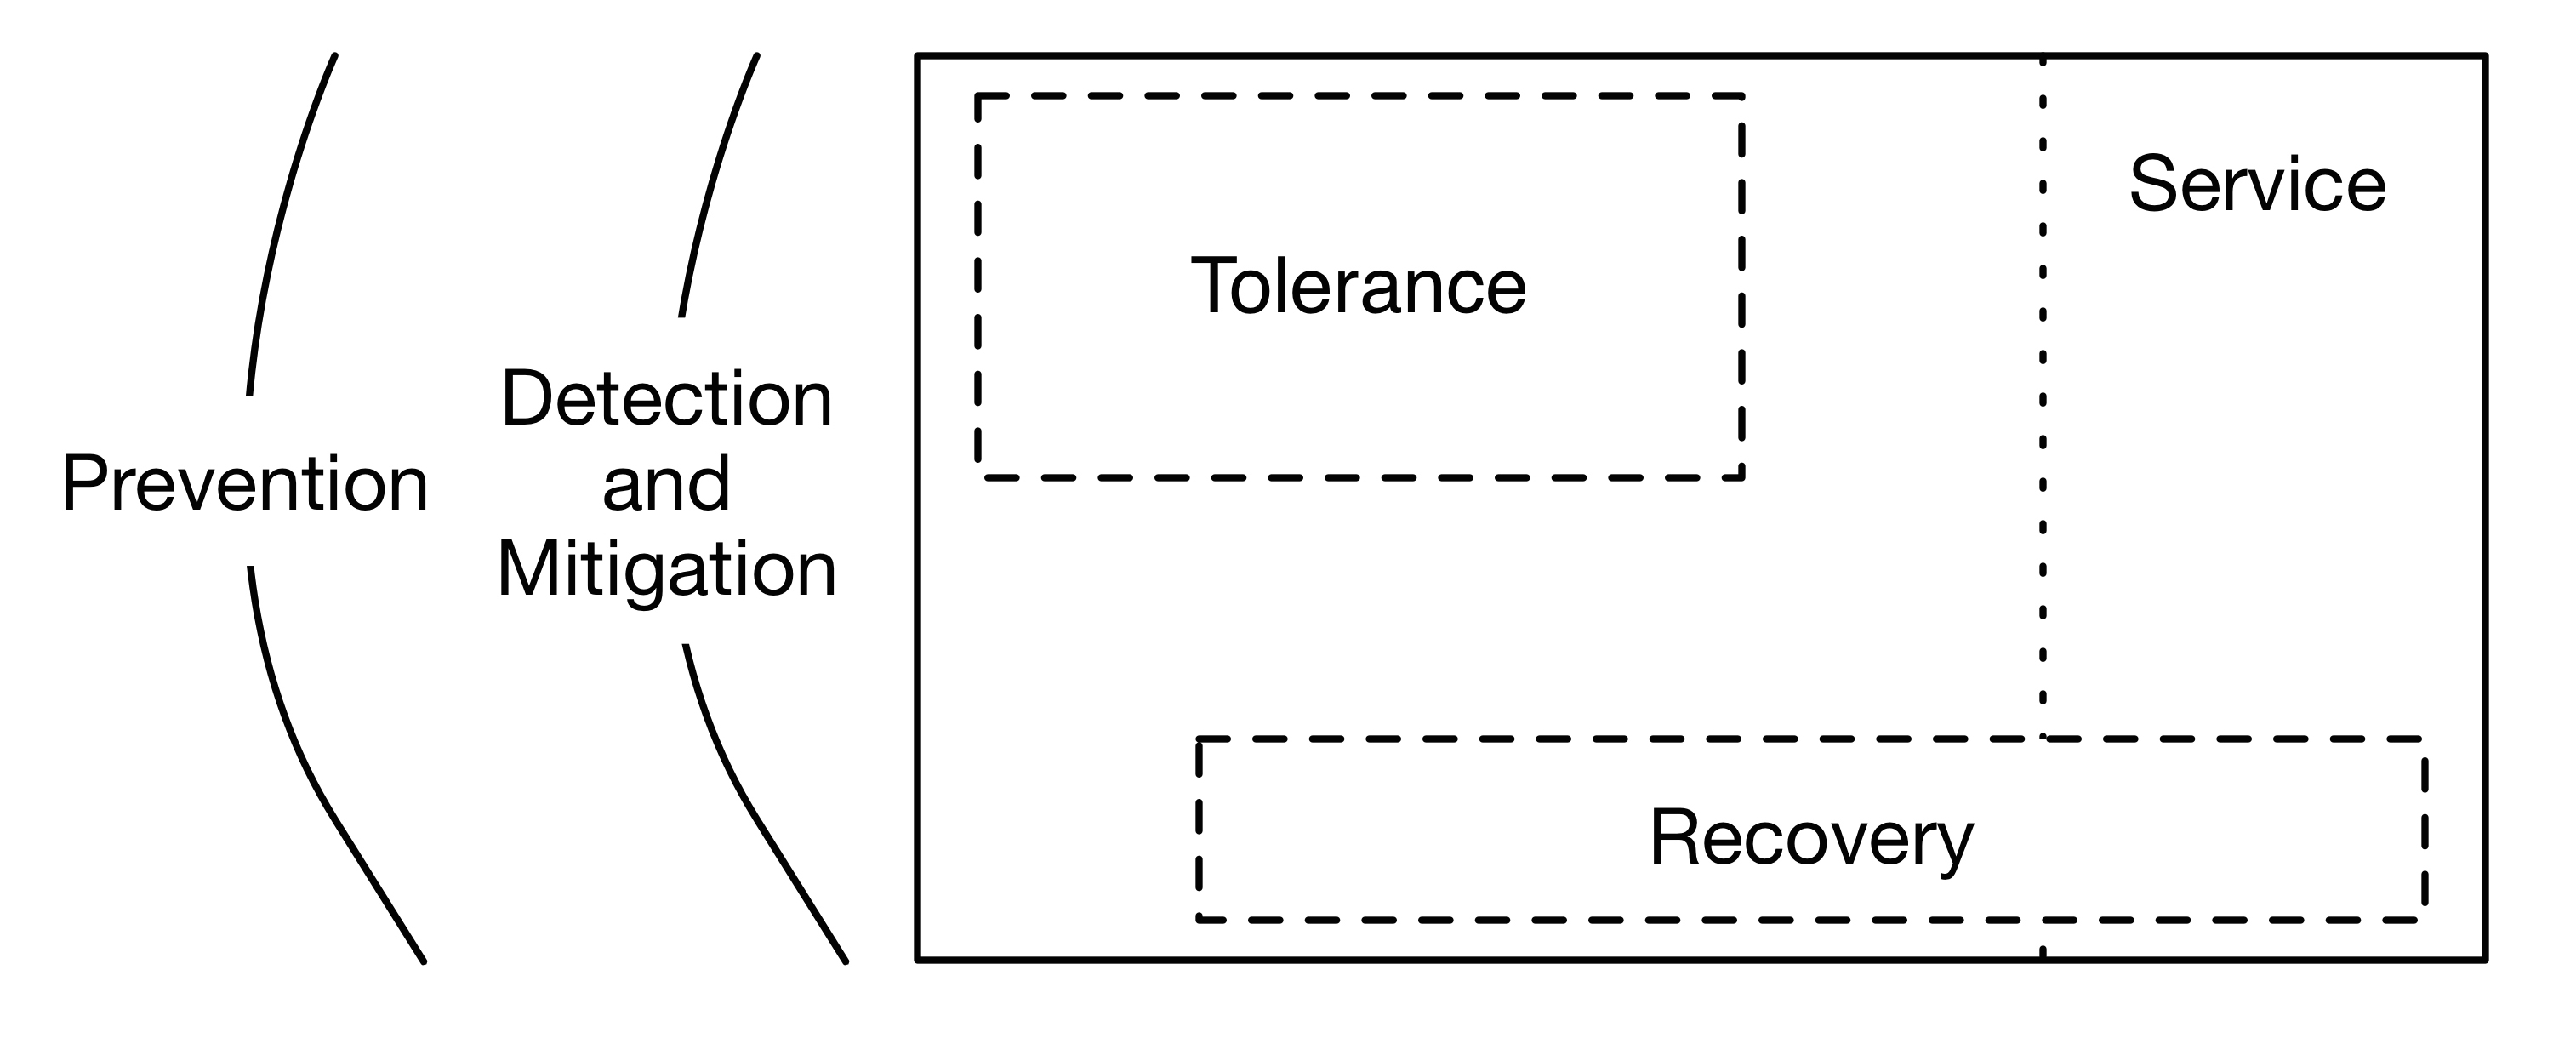
\includegraphics[width=0.7\textwidth]{img/ie0}
		 \end{figure}
	\end{center}
	\note{
	No entanto estes mecanismos são penetrados por ataques devido a novas vulnerabilidades no software e a novos métodos de ataque. Além disso, os administradores e utilizadores podem cometer erros acidentalmente ou maliciosamente na configuração ou utilizacação do sistema e, através de pedidos que são legitimos, corromper os dados da aplicação.
	Neste caso, além dos mecanismos de prevenção e detecção serem ultrapassados, os mecanismos de tolerancia vão replicar os dados corrompidos afectando todas as réplicas porque se tratam de pedidos legitimos e não de mensagens bizantinas.	      
	}
\end{frame}

%%%%%%%%%%
% 02:45
%%%%%%%%%%%%%
%-------------------------------------------------------------------
	
\begin{frame}[c]{Motivation}
	\begin{center}
	{\Large \textbf{Intrusions and failures happen!}} 
	\vspace{20pt}
		\begin{figure}
			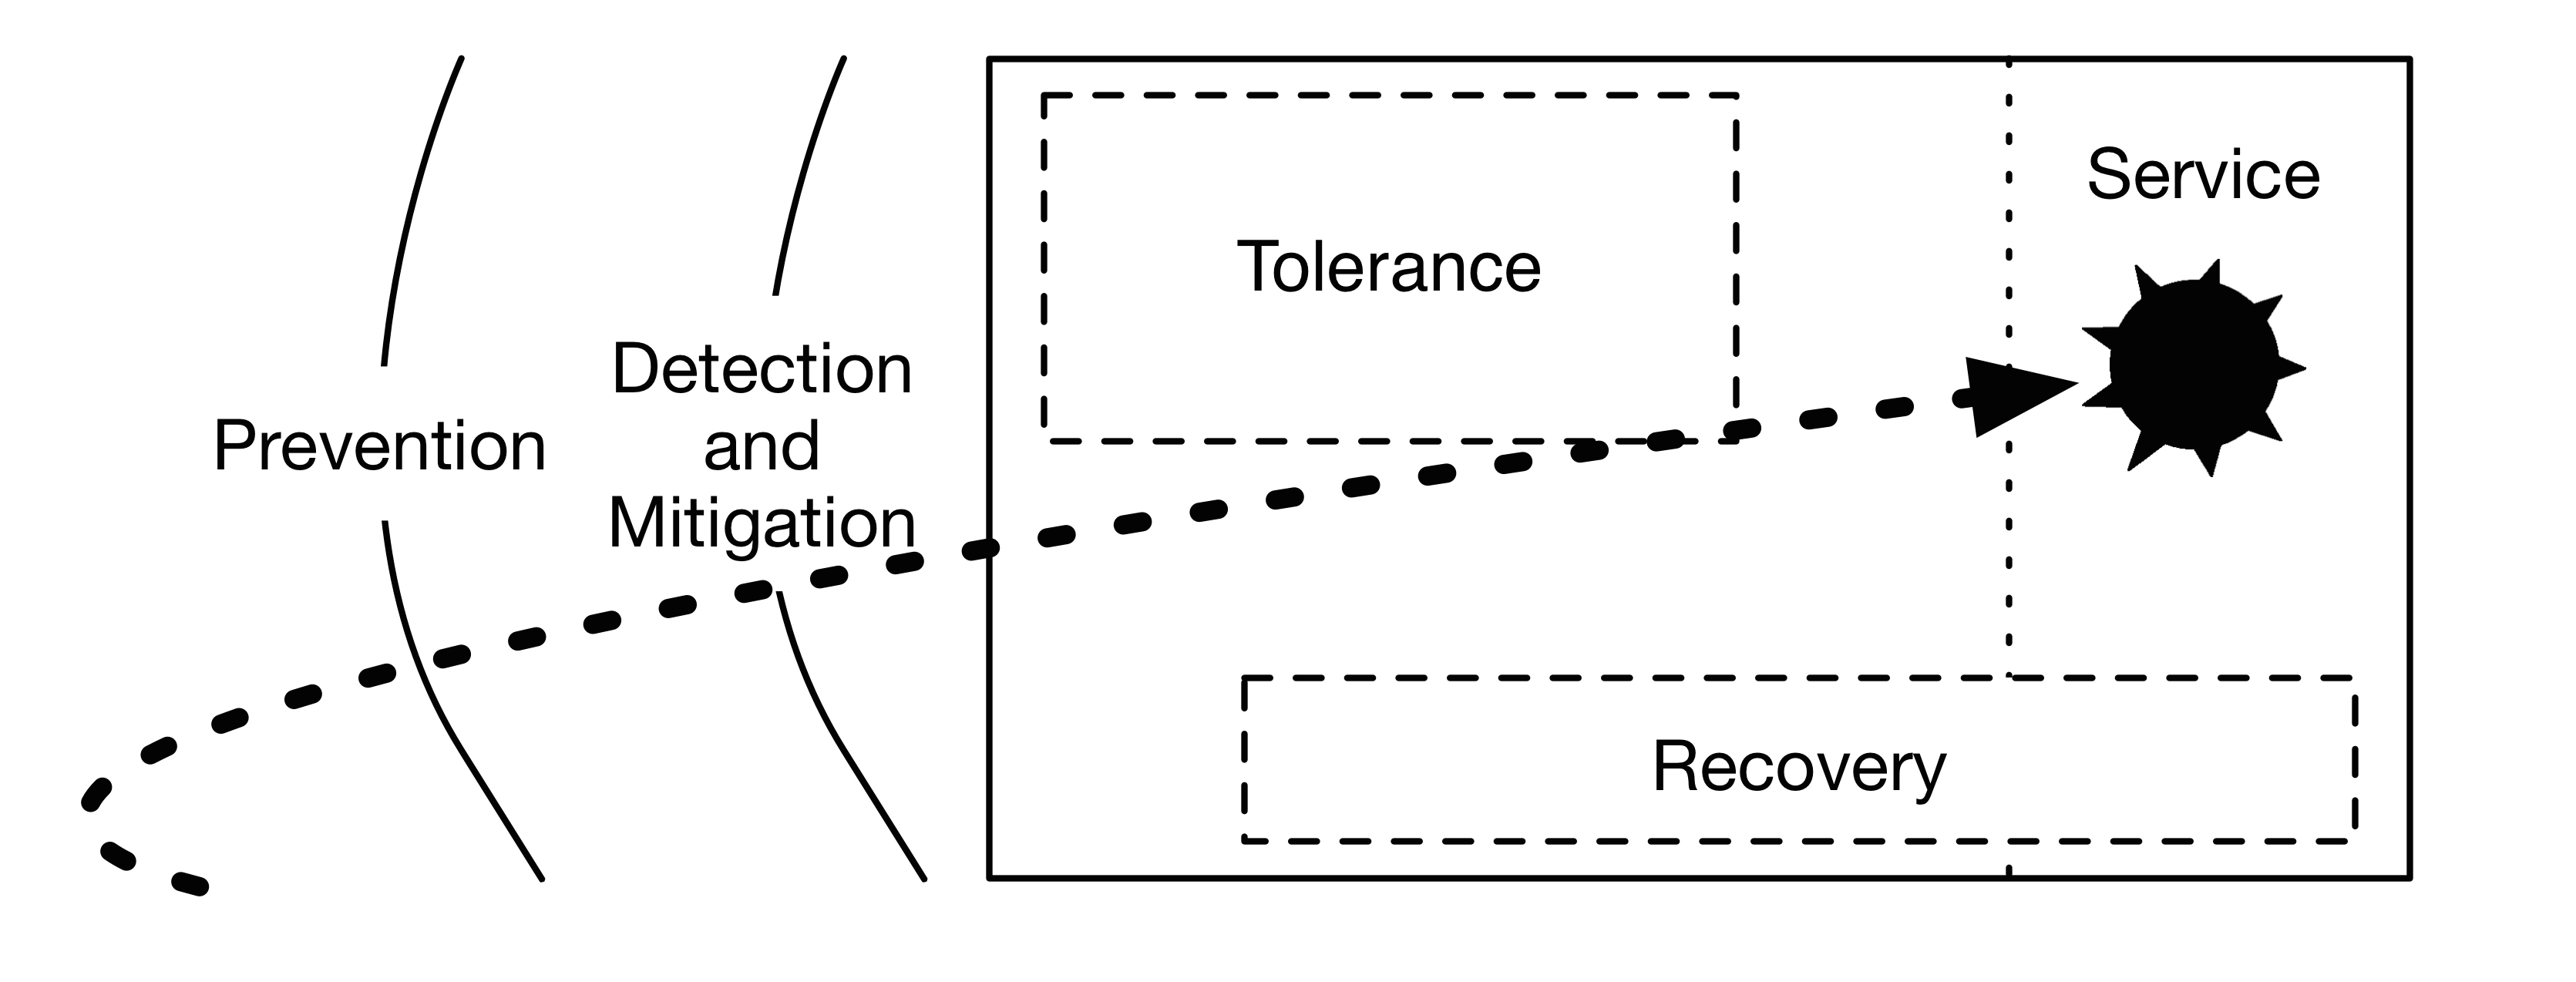
\includegraphics[width=0.8\textwidth]{img/ie4}
		\end{figure}	
	\end{center}
	\note{
	Como o nosso exemplo simples provou, as barreiras de segurança podem ser ultrapassadas. Haveriam muitos outros exemplos possíveis mas este em particular não só é frequente como também pode ser um simples erro do utilizador.
	Por isso, as intrusões podem acontecer.
	}
\end{frame}
%--------------------- Goals -----------------------------------
\begin{frame}[c]{Problem statement}
 \begin{center}
	{\Large How to recover from intrusions in PaaS?}
	\end{center}
	\note{
	Assim sendo, como podemos recuperar das intrusões?
	}
\end{frame}

%-----------------------------------------
\section{Related Work}
\begin{frame}[t]{Goals}
      \vskip-0.5cm
      \textbf{Accept intrusions and remove their effects}
      \vskip0.5cm
		\begin{itemize}
			\item Identify the intrusion effects
			\item Remove intrusion effects
			\item Recover the application integrity
			\item Tolerate intrusions: recovery without exposing downtime	\footnote{Does not replace the prevention and tolerance}

			\item Recover from user and administrator mistakes
		\end{itemize}
		\note{
		Ou seja, como podemos aceitar intrusões e remover os seus efeitos? O ideal seria conseguir determinar quais foram os efeitos da intrusão, remove-los e recuperar a integridade da aplicação. Como extra, se conseguissemos fazer isto sem que a aplicação se torne indisponível para os utilizadores, então teriamos um sistema tolerante a intrusões. Como extra, também poderiamos recuperar de erros dos utilizadores e administradores. São exactamente estes os objectivos dos serviços recuperação de intrusões. Vejamos como é o processo de recuperação nos sistemas actuais.
		}
\end{frame}


%---------------------Related Work-----------------------------------
\begin{frame}[t]{1. Identification of intrusion effects}
  \textbf{Goal:} Identify the intrusion actions or objects
  \vspace{2ex}
  \begin{itemize}
    \item IDS: {\footnotesize \textit{[Taser,ITDB,Phoenix,Retro,Dare,Goel et al., Undo for Operators]}}
    \item Software update {\footnotesize \textit{[Warp,Aire]}} 
  \end{itemize}
    
\note{
O processo de recuperação começa após o administrador determinar um conjunto de dados ou acções que foram afectados. Os administradores podem ser apoiados por sistemas de detecção a intrusões. Em alternativa, podem realizar um update ao software da aplicação para resolver uma vulnerabilidade.
} 
\end{frame}


%------------------------------

\begin{frame}[c]{1. Identification of intrusion effects}
	\begin{center}
		\begin{figure} 
			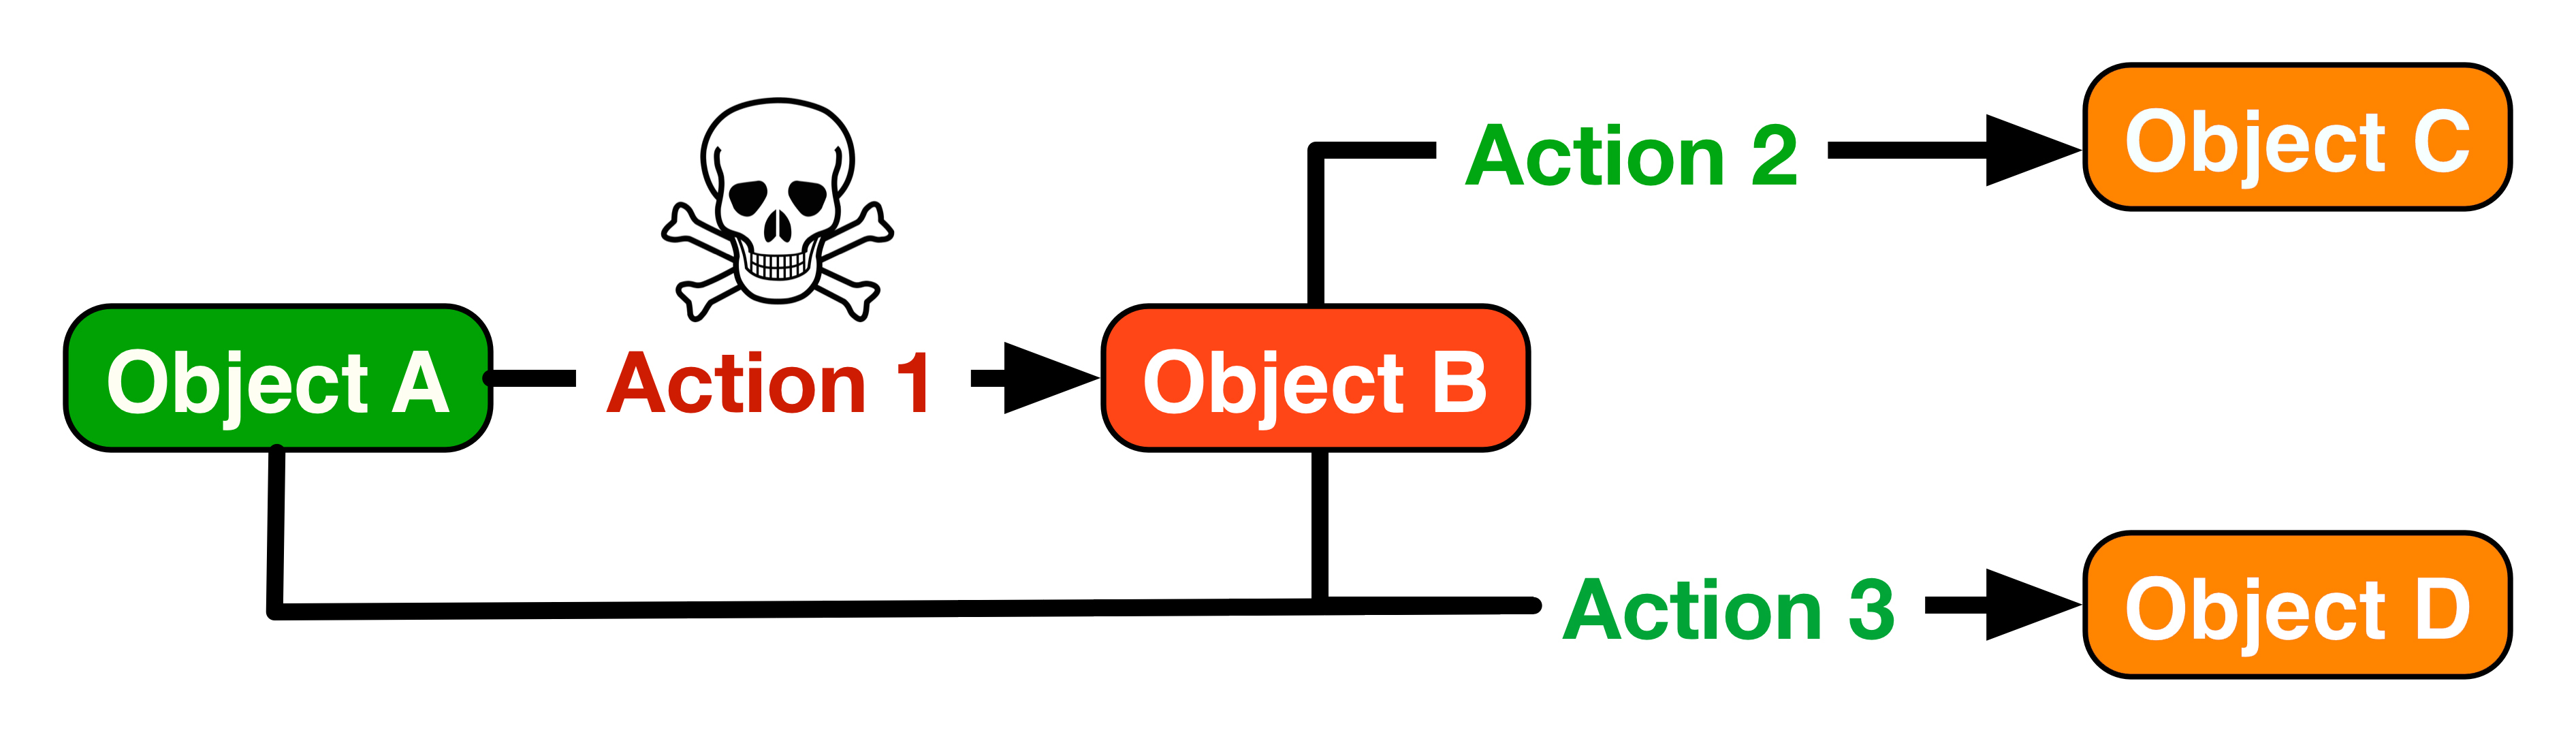
\includegraphics[width=0.8\textwidth]{img/propagation}
			\end{figure}
	\end{center}
\note{
Partindo dos dados fornecidos pelo administrador, os serviços de recuperação determinam quais os objectos e pedidos  afectados. 
Ou seja, se criarmos um grafo em que os nós são objectos e os vertices são as acções que lêem um objecto e escrevem outro, verificamos que as acções são interdependentes através dos objectos. 
Por exemplo, se acção 1 foi um ataque, então o objecto B foi afectado. Por isso, remover os efeitos da intrusão implica remover o valor que a acção 1 escreveu no objecto B.
} 
\end{frame}

%------------------------------


\begin{frame}[t]{2. Remove intrusion effects}
		\begin{itemize}
	\item Versioning {\footnotesize \textit{[Phoenix, Warp,Aire]}}
	\item Snapshot {\footnotesize \textit{[Taser, Retro,Date, Undo for Operators]}}
	\item Compensation {\footnotesize \textit{[Goel et al,ITDB]}}
		\end{itemize}
		\vskip1cm
		\begin{center}
		  \textbf{storage vs computing}
		\end{center}
		\note{
		Existem 3 alternativas para remover os efeitos:
		- Podemos carregar a versão do objecto imediatamente anterior ao ataque.
		- Podemos carregar um snapshot do sistema e refazer as operações legitimas até ao momento da intrusão
		- Ou então inverter todas as acções realizadas sobre o objecto desde o momento presente até ao momento anterior à intrusão.

		Cada uma destas propostas tem vantagens e desvantagens. De cima para baixo, ordenadas pelo espaço ocupado em disco e de baixo para cima ordenadas pelo número de acções que temos de repetir para um valor.
		}
\end{frame}


%----------------------------------------
\begin{frame}[t]{3. Recover the application integrity}
		\begin{center}
			\vskip-20pt
		\begin{figure} 
			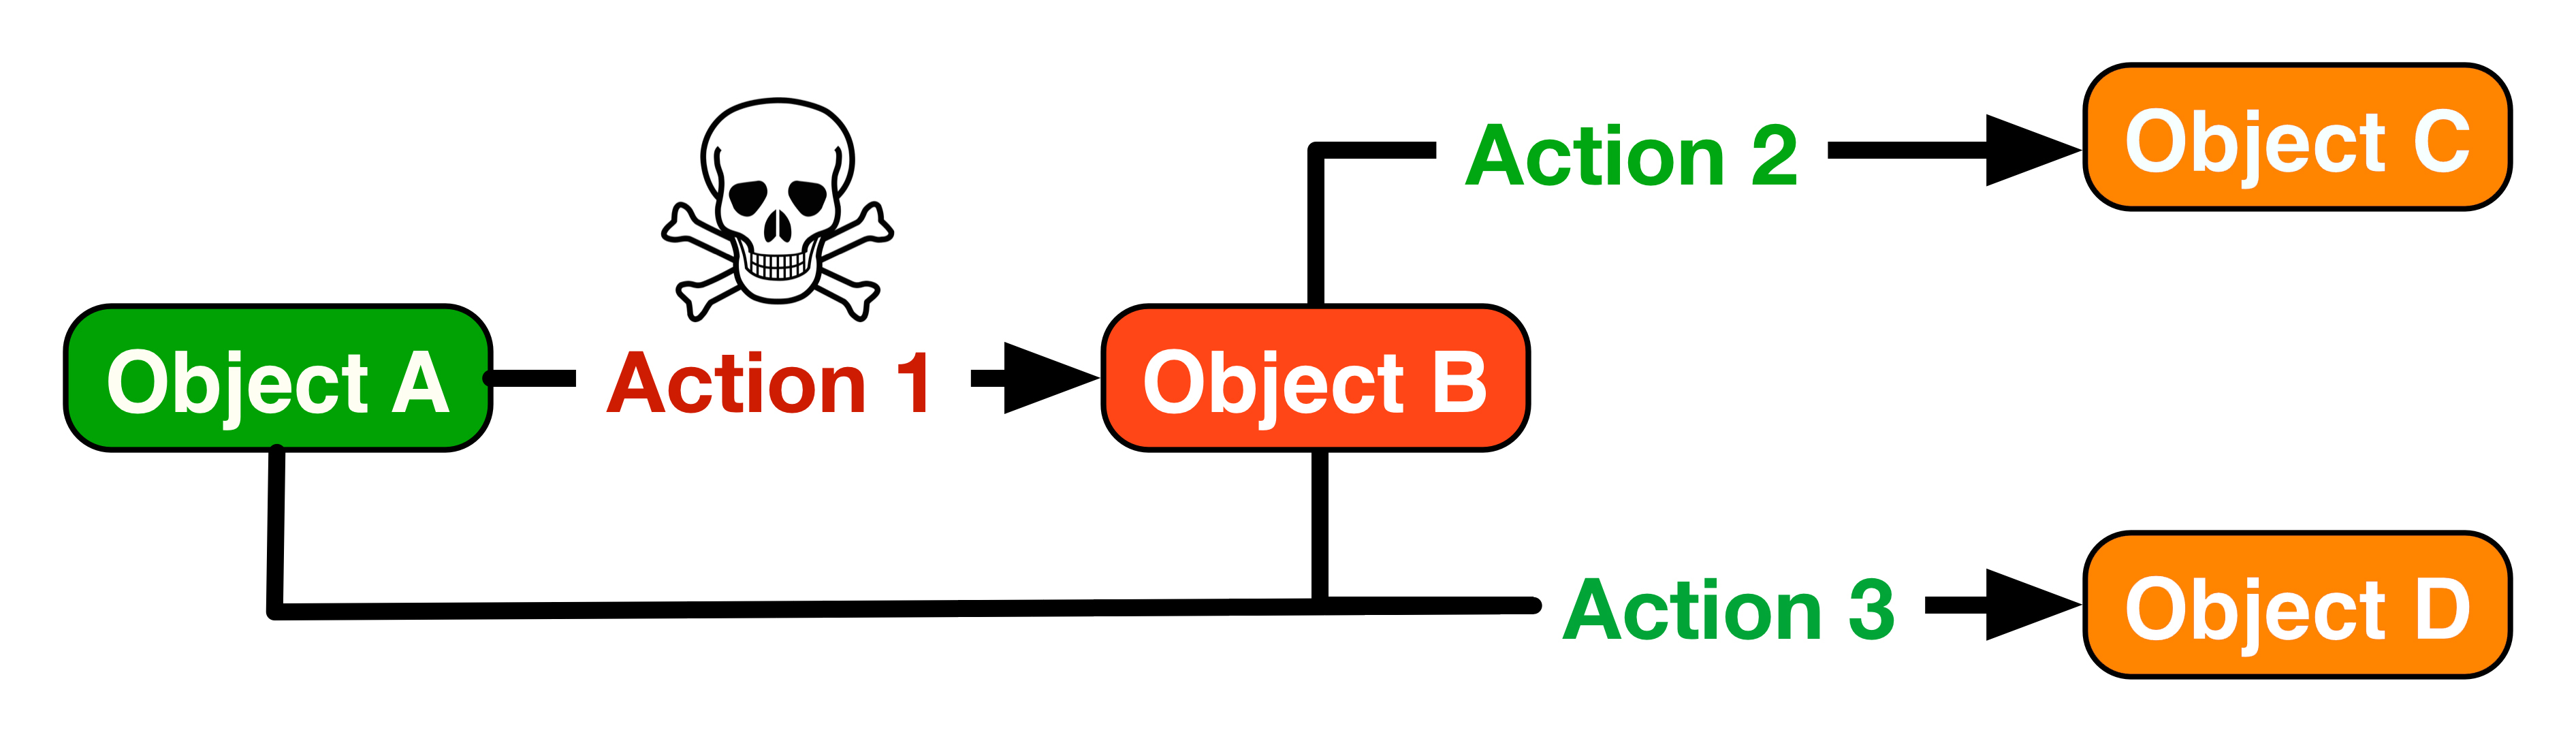
\includegraphics[width=0.8\textwidth]{img/propagation}
			\end{figure}
		\end{center}
	\begin{itemize}
		\item No replay {\footnotesize \textit{[Taser, ITDB, Phoenix]}}
		\item Taint via replay {\footnotesize \textit{[Retro,Dare,Goel et al,Warp,Aire]}}
		\item Replay all {\footnotesize \textit{[Undo for Operators]}}
	\end{itemize}

\note{
Vejamos agora o grafo de dependencias de novo. Mesmo que removamos o objecto B, o ataque continua a ter efeitos. Os objectos C e D foram influênciados, tainted, porque leram o valor errado do objecto B. Alguns dos projectos apresentados limitam-se a remover também os objectos C e D. Esta abordagem é insuficiente porque continua a penalizar os utilizadores legitimos.

Outros, removem apenas o valor do objecto B mas voltam a executar as acções 2 e 3 e caso os objectos C e D sejam agora diferentes, vão re-executar as acções que leiam destes objectos também. Este ciclo é recursivo. Neste caso, o sistema recupera um estado consistente e os utilizadores já não são penalizados.

No entanto, podem haver dependências indirectas que não são determinadas pelo grafo. Por isso, um dos trabalhos apresentados propõe realizar todos as acções legitimas. Neste caso, o sistema carrega uma cópia anterior à intrusão do objecto B e refaz as acções 2 e 3 e todas as seguintes, de modo ordenado.
} 
%marcar os tainted
\end{frame}

%-------------------------------------------------------------
\begin{frame}[t]{Recovery: Where?}
		\begin{itemize}
	\item Operating system {\footnotesize \textit{[Taser,Retro]}}:
	\begin{itemize}
			\item System calls, files and sockets
	\end{itemize}
	\item Database {\footnotesize \textit{[ITDB,Phoenix]}}:
	\begin{itemize}
		\item Read and write sets: table, table block, row or field
	\end{itemize}
	\item Web Applications{\footnotesize \textit{[Goel et al, Warp,Aire,Undo for Operators]}}:
		\begin{itemize}
		\item User requests and database transactions
		\end{itemize}
	\end{itemize}


\note{
O modo de estabelecer os vertices do grafo que definem as dependencias, depende da camada da aplicação que queremos recuperar. As propostas para File System Recovery baseiam-se em dependências estabelecidas pelas system calls realizadas pelos processos interligando objectos como os ficheiros e sockets. 
No caso das base de dados, as dependências são estabelecidas pelos valores que a transacção lê e escreve.
No caso da aplicação, que geralmente são suportadas por bases de dados, as dependências são estabelecidas não só pelas regras das bases de dados como também pela camada aplicacional. A camada aplicacional pode usar um transacção para gerar os valores da transação seguinte.
 } 
\end{frame}
%---------------------------------------------------------------------
\section{Proposed Solution}
\begin{frame}[t]{Problems}
	\begin{itemize}
		\item \textbf{Scalability}
		\begin{itemize}
		  \item Single database and server
		\end{itemize}
		\item \textbf{Integration}
		\begin{itemize}
		  \item Lack of generic application support
		  \item Configuration per application
		\end{itemize}
		\item \textbf{Application downtime}
	\end{itemize}
\note{
Contudo as soluções actuais não têm em conta o novo paradigma de cloud. As soluções visam apenas sistemas constituidos por uma unica maquina no caso do OS, uma base de dados transacional ou no caso das webapps apenas um servidor e uma database transacional. Isto não só não é escalável para as novas aplicações web como também incorre do problema de que caso o sistema seja atacado, o sistema de recuperação está vulnerável. Mais, as soluções actuais exigem que os administradores de sistema instalem e configurem o sistema para cada aplicação. Visto que os administradores de sistemas, enquanto humanos, cometem erros e que estes sistemas raramente são testados, configurar um serviço de recuperação para cada aplicação é um risco.
A maioria das soluções actuais requer que a aplicação seja desligada para que o sistema possa recuperar das intrusões e isso pode ter custos elevados.
} 
\end{frame}

%---------------------------------------------------------------------------

%----------------------
\subsection{Goals}
\begin{frame}[t]{Project Goals}
	\textbf{Shuttle: Intrusion recovery service for PaaS}
	\vspace{10pt}
	\begin{itemize}
	\item PaaS Integration
		\begin{itemize}
		\setlength{\wideitemsep}{0.3cm}
		\item Standard architecture for Web Applications  
		\item Service-oriented database access through provided libraries
		\item Service available without setup and configuration 
		\end{itemize}
	\item NoSQL databases
	\end{itemize}
	\note{
	Tendo em conta estes problemas, apresentamos Shuttle. Shuttle é um serviço para Platform as a Service que permite aos developers recuperar as suas applicações sem terem de criar, instalar e configurar um sistema de recuperação de intrusões. Mais, dado o ambiente de Platform as a Service, este serviço suporta multiplas instâncias aplicacionais ou de bases de dados, resolvendo os problemas de escalabilidade das soluções actuais. As capacidades computacionais e de storage da Cloud são uma excelente opção para recuperar as aplicações porque disponibiliza um número virtualmente ilimitado de instâncias para executar o processo de recuperação e que são pagas apenas durante a sua utilização.

	Mais, o modelo PaaS tem uma arquitectura padrão que é partilhada pelas várias aplicações e as bases de dados são acedidas através de bibliotecas disponibilizadas pelos providers.

	Outro objectivo, é integrar o Shuttle numa base de dados NoSQL para que possa escalar e servir várias aplicações em simultanêo.

}
\end{frame}

%----------------------
\begin{frame}[t]{Project Goals}
	Remove the effects of:    \\
	\vspace{2ex}
	\begin{itemize}
	\item Software flaws
	\item Corrupted requests and data
	\item Intrusions in PaaS instances
	\end{itemize}
	\note{
	O Shuttle irá portanto remover os efeitos de falhas de software, pedidos e dados corrompidos e ainda remover as intrusões que existem dentro dos containers de PaaS em que o software corre, por exemplo: máquinas virtuais.
	}
\end{frame}

%----------------------
\begin{frame}[t]{Project Goals}
	\begin{itemize}
	\item Support software updates
	\item Low runtime overhead
	\item NoSQL database snapshot
	\item Recover without stopping the application
	\end{itemize}
	\note{
	Para isso, a nossa proposta irá ainda suportar actualizações de software, por exemplo para corrigir vulnerabilidades. Para que seja utilizável, irá ter um overhead minimo na execução do sistema, realizar snapshots da base de dados para reduzir o número de acções a re-executar e conseguir recuperar sem ter de parar a execução da aplicação.
	}
\end{frame}


\include{sections/E-architecture}
%-------------------------------------------------------------------
\subsection{Evaluation}
\begin{frame}[t]{Evaluation}
	\begin{itemize}
	 \item \textbf{Prototype:} Java Servlet (Spring Framework) version of Question \& Answers System
	 \item \textbf{Data:} Data crawled from Stackoverflow.com	 	 \item \textbf{Database: }Cassandra and Voldemort (Key-Value store, DynamoDB)
	 \item \textbf{PaaS: }OpenShift, AppScale (Google App Engine) 
	 \item \textbf{IaaS: } OpenStack and Amazon Web Services or Google Cloud Platform
	\end{itemize}    
\note{
Este conceito será testado com uma aplicação protótipo Java Spring baseada num sistema de Question and Answers. Serão usados PaaS opensource Openshift e AppScale. Os pedidos serão guardados na Big Table Cassandra enquanto que a aplicação usará o Voldemort, um key-value store da LinkedIn equivalente ao DynamoDB da Amazon.
}
\end{frame}

\begin{frame}[t]{Evaluation}
	\begin{itemize}
	\item \textbf{Record impact:} Delay, throughput, resource usage, maximum load
	\item \textbf{Replay:} Precision, recall, duration and scalability
	\item \textbf{Integrity and Availability:} Corrupted and unavailable data during recovery
	\item \textbf{Concurrency: }Correctness and performance improvement
	\item \textbf{Cost: }Monetary cost in a public cloud provider
	\end{itemize}
	
\note{
Iremos medir qual o impacto do serviço na aplicação, qual a precisão, recall, duração e escalabilidade do processo de replay. Iremos avaliar se a aplicação consegue permanecer integra e disponivel durante o processo, se o processo de replay em parallel é efectivamente vantajoso e qual o custo de usar esta solução num cloud provider.
} 
\end{frame}
%-------------------------------------------------------------------
\section{Conclusion}
\subsection{Schedule}
\begin{frame}[c]{Schedule}
\vskip-5mm
\makebox[\linewidth][c]{
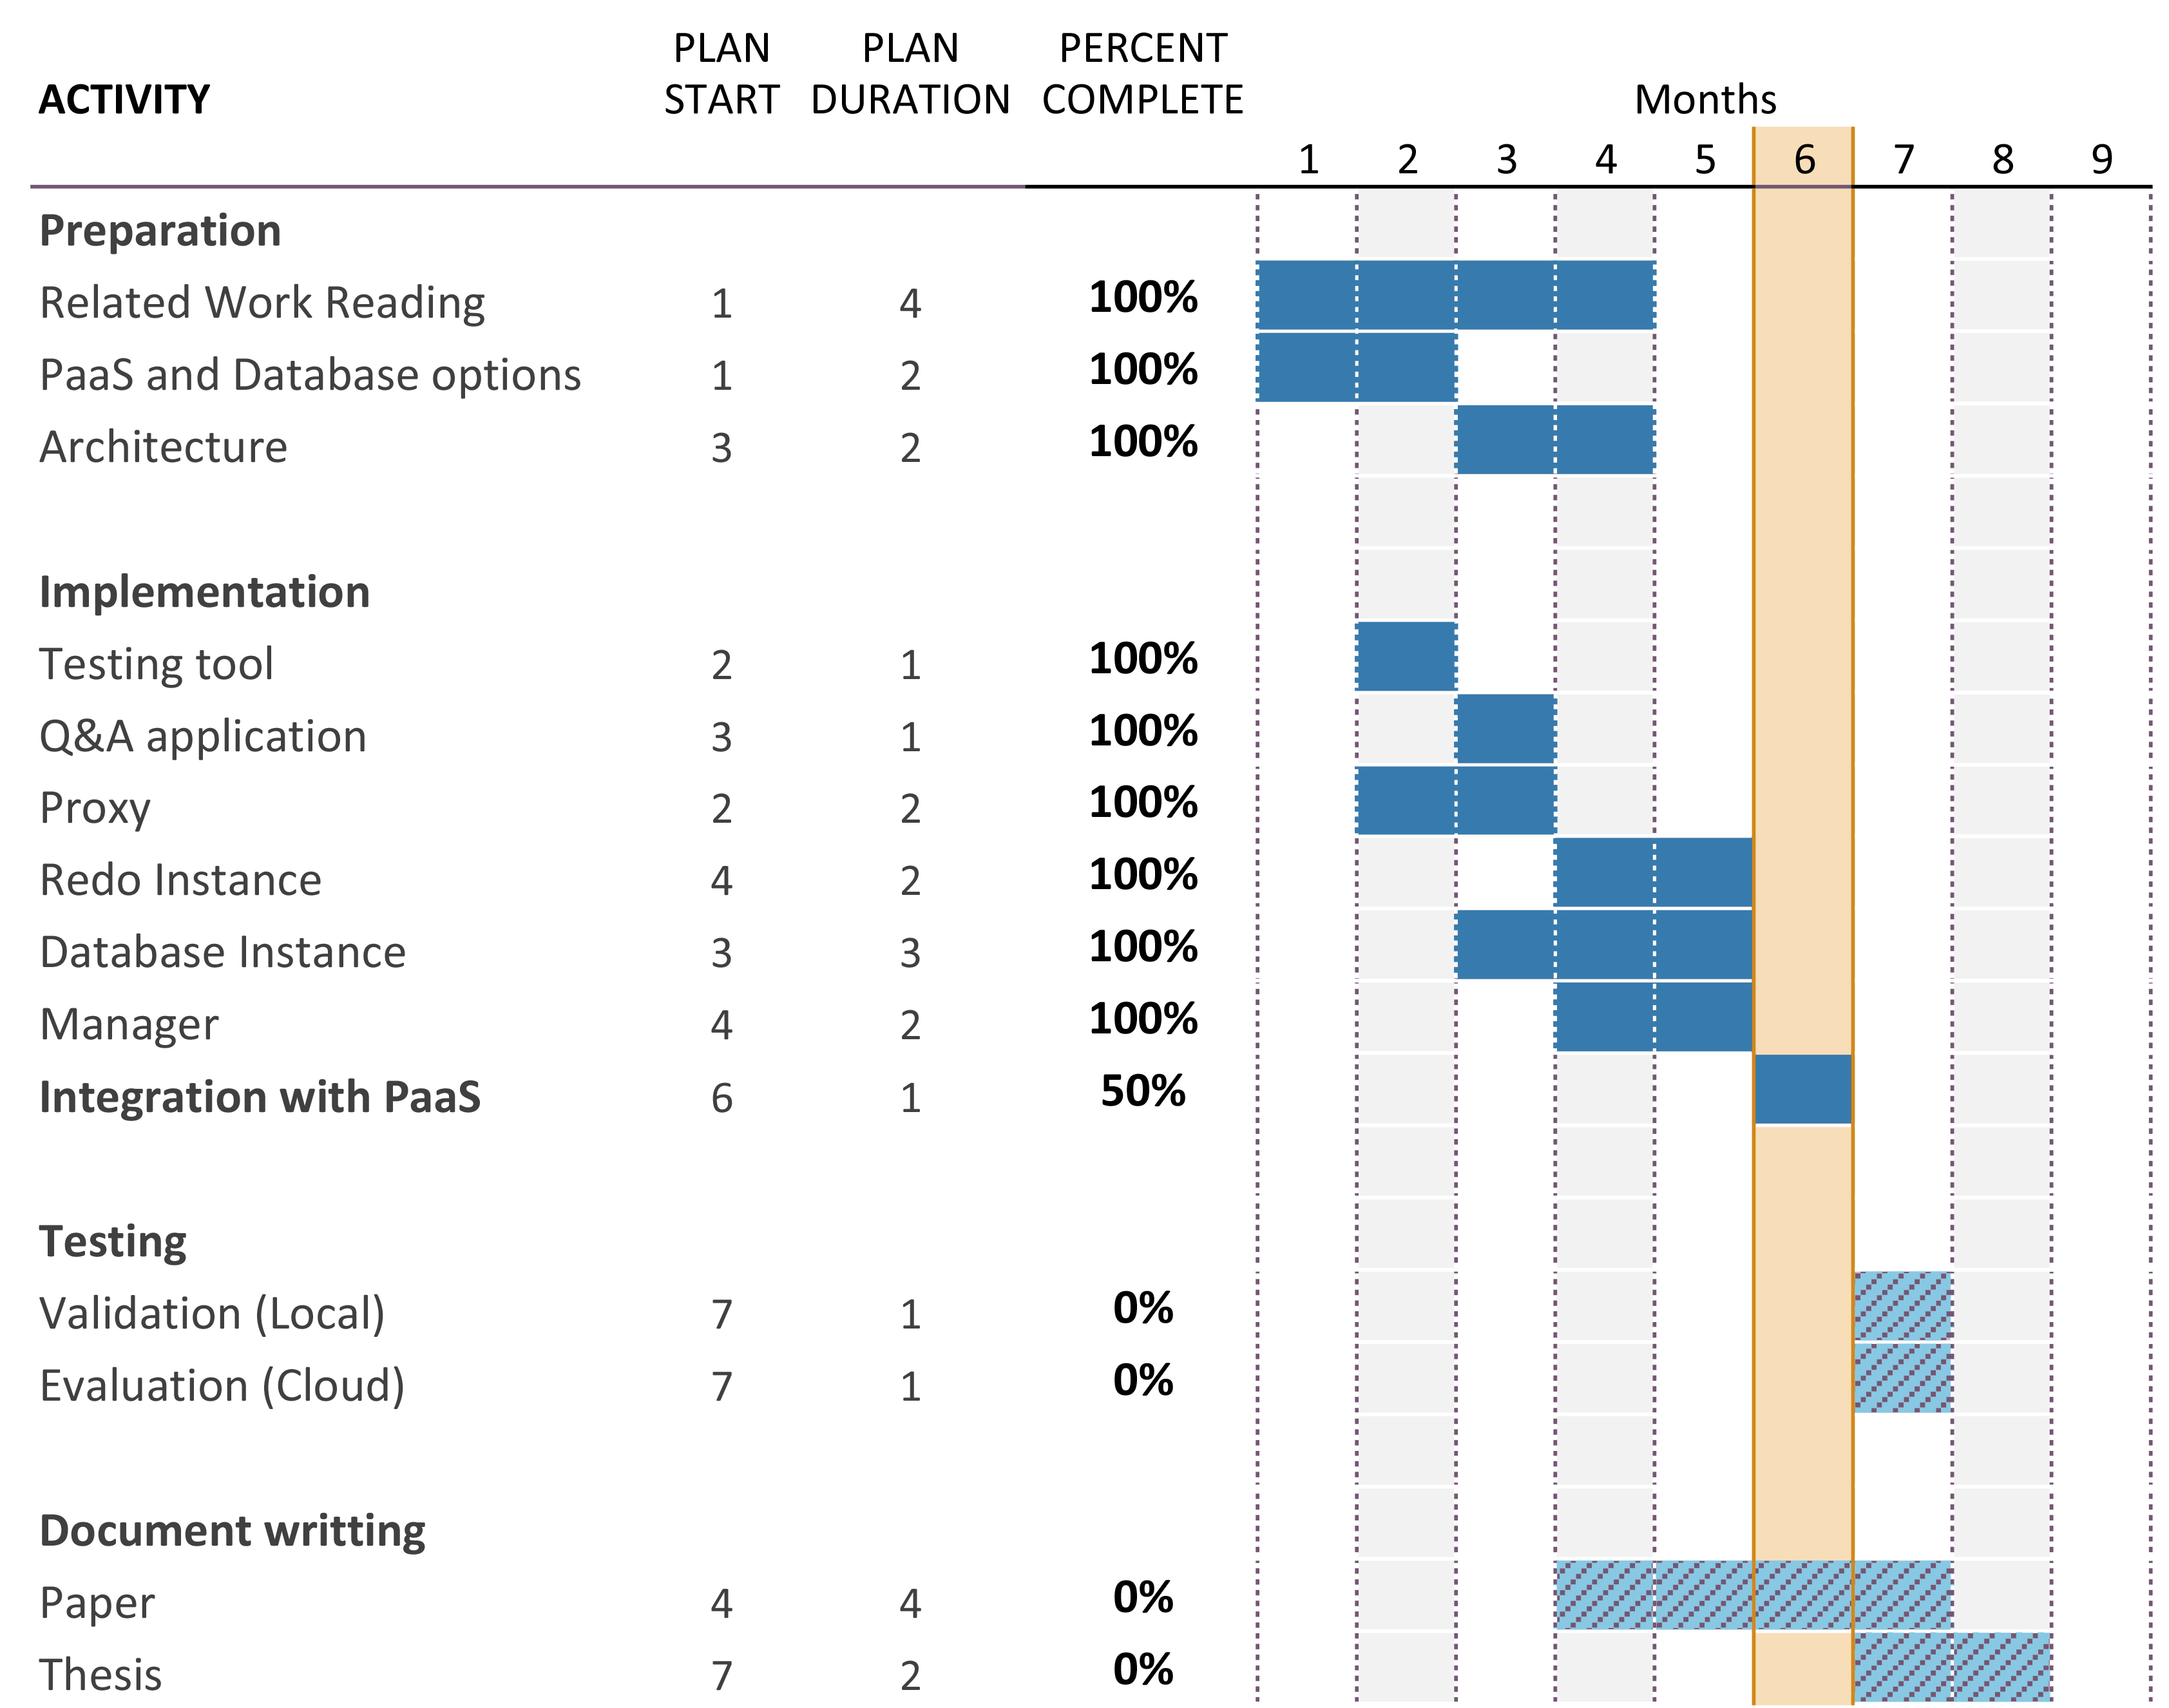
\includegraphics[width=90mm]{img/gantt}
}

\note{
Na fase de preparação comecei por ler e analisar o trabalho relacionado, as opções e arquitectura para PaaS e base de dadoss e fiz uns pequenos testes de conceito usando Python.
} 
\end{frame}



%-------------------------------------------------------------------

\subsection{Conclusion}

\begin{frame}[c]{Conclusion}
    \vskip-0.5cm
	\textbf{Shuttle is the first:}
	\begin{itemize}
	  \setlength{\wideitemsep}{0.3cm}
	  \item  Intrusion recovery service for PaaS using replay
	  \item  To NoSQL databases and snapshoting
	  \item  To concern the parallel replay
	\end{itemize}
	\vskip0.5cm
	\textbf{Amongst the first:}
	\begin{itemize}
	  \setlength{\wideitemsep}{0.3cm}
	  \item  To incorporate the instance renewing
	  \item  To recover without application downtime
	\end{itemize}
	
\note{
Como proposto, o sistema apresentado guarda os pedidos dos utilizadores e as suas dependências para remover os ataques a aplicações deployed em Paas. Mais, conseguimos suportar actualizações de software ou migrar a aplicação para containers limpos.
Pelo que investigámos, este é o primeiro sistema de recuperação para PaaS e o primeiro projecto que aborda o paralelismo do replay e o seu uso em bases de dados não SQL.
Acredito portanto que este sistema apresenta um grande potencial para a comunidade.
} 
\end{frame}

\begin{frame}[t,c]{}
  \begin{center}
  \Huge  Thank you for your attention
  \end{center}
  \note{Muito obrigado pela vossa atencao, estou agora disponivel para questoes}
\end{frame}
\end{document}

